%%% LaTeX Template: Designer's CV
%%%
%%% Source: http://www.howtotex.com/
%%% Feel free to distribute this template, but please keep the referal to HowToTeX.com.
%%% Date: March 2012


%%%%%%%%%%%%%%%%%%%%%%%%%%%%%%%%%%%%%
% Document properties and packages
%%%%%%%%%%%%%%%%%%%%%%%%%%%%%%%%%%%%%
\documentclass[a4paper,12pt,final]{memoir}

% misc
\renewcommand{\familydefault}{bch}	% font
\pagestyle{empty}					% no pagenumbering
\setlength{\parindent}{0pt}			% no paragraph indentation

% cvsection settings
\usepackage{titlesec}
\usepackage{titling}

% section
\titleformat{\section}
{\Large \bfseries}
{}
{.25em}
{}[\titlerule]

% cvsubsection
\titleformat{\subsection}
{\bfseries \color{RoyalBlue}}
{}
{0em}
{}

% cvsubsubsection
\titleformat{\subsubsection}[runin]
{}
{}
{0em}
{}[ --]

\titlespacing{\section}
{0em}{1.5em}{.5em}

\titlespacing{\subsection}
{0em}{1em}{.25em}

\titlespacing{\subsubsection}
{0em}{.25em}{.5em}

% required packages (add your own)
\usepackage{flowfram}										% column layout
\usepackage[top=1cm,left=1cm,right=1cm,bottom=1cm]{geometry}% margins
\usepackage{graphicx}										% figures
\usepackage{url}											% URLs
\usepackage[usenames,dvipsnames]{xcolor}					% color
\usepackage{multicol}										% columns env.
	\setlength{\multicolsep}{0pt}
\usepackage{paralist}										% compact lists
\usepackage{tikz}
\usepackage{attachfile}

\graphicspath{{C:/Users/LAB5892A/Desktop/outgoing/figures/}}
%%%%%%%%%%%%%%%%%%%%%%%%%%%%%%%%%%%%%
% Create column layout
%%%%%%%%%%%%%%%%%%%%%%%%%%%%%%%%%%%%%
% define length commands
\setlength{\vcolumnsep}{\baselineskip}
\setlength{\columnsep}{\vcolumnsep}

% frame setup (flowfram package)
% left frame
\newflowframe{0.2\textwidth}{\textheight}{0pt}{0pt}[left]
	\newlength{\LeftMainSep}
	\setlength{\LeftMainSep}{0.2\textwidth}
	\addtolength{\LeftMainSep}{1\columnsep}
 
% small static frame for the vertical line
\newstaticframe{1.5pt}{\textheight}{\LeftMainSep}{0pt}
 
% content of the static frame
\begin{staticcontents}{1}
\hfill
\tikz{%
	\draw[loosely dotted,color=RoyalBlue,line width=1.5pt,yshift=0]
	(0,0) -- (0,\textheight);}%
\hfill\mbox{}
\end{staticcontents}
 
% right frame
\addtolength{\LeftMainSep}{1.5pt}
\addtolength{\LeftMainSep}{1\columnsep}
\newflowframe{0.7\textwidth}{\textheight}{\LeftMainSep}{0pt}[main01]


%%%%%%%%%%%%%%%%%%%%%%%%%%%%%%%%%%%%%
% define macros (for convience)
%%%%%%%%%%%%%%%%%%%%%%%%%%%%%%%%%%%%%
\newcommand{\Sep}{\vspace{1.5em}}
\newcommand{\SmallSep}{\vspace{0.5em}}

%\newenvironment{AboutMe}
%	{\ignorespaces\textbf{\color{RoyalBlue} About me}}
%	{\Sep\ignorespacesafterend}
	
%\newcommand{\CVSection}[1]
%	{\Large\textbf{#1}\par
%	\SmallSep\normalsize\normalfont}

%\newcommand{\CVItem}[1]
%	{\textbf{\color{RoyalBlue} #1}}

\definecolor{antiquewhite}{rgb}{0.98, 0.92, 0.84}
\definecolor{antiquewhited}{rgb}{0.49, 0.46, 0.42}	
	
\newcommand{\wheelchart}[6]{
	
    % Calculate total
    \pgfmathsetmacro{\totalnum}{0}
    \foreach \value/\colour/\name in {#1} {
        \pgfmathparse{\value+\totalnum}
        \global\let\totalnum=\pgfmathresult
    }

    \begin{tikzpicture}
      % The text in the center of the wheel
      \node[align=center,text width=2*#3]{#2};

      % Calculate the thickness and the middle line of the wheel
      \pgfmathsetmacro{\wheelwidth}{#4-#3}
      \pgfmathsetmacro{\midradius}{(#4+#3)/2}

      % Rotate so we start from the top
      \begin{scope}[line width=\wheelwidth,rotate=90]

      % Loop through each value set. \cumnum keeps track of where we are in the wheel
      \pgfmathsetmacro{\cumnum}{0}
      \foreach \value/\colour/\name in {#1} {
            \pgfmathsetmacro{\newcumnum}{\cumnum + \value/\totalnum*360}

            % Calculate the percent value
            \pgfmathsetmacro{\percentage}{\value/\totalnum*100}
            
            % Calculate the mid angle of the colour segments to place the labels
            \pgfmathsetmacro{\midangle}{-(\cumnum+\newcumnum)/2}

			% This is necessary for the labels to align nicely
			\pgfmathparse{
				(-\midangle<180?"west":"east")
			} \edef\textanchor{\pgfmathresult}
			\pgfmathsetmacro\labelshiftdir{1-2*(-\midangle>180)}

            % Draw the color segments. Somehow, the \midrow units got lost, so we add 'pt' at the end. Not nice...
            \draw[\colour] (-\cumnum:\midradius pt) arc (-\cumnum:-(\newcumnum):\midradius pt);

            % Draw the data labels
            \node at (\midangle:#4 + 1ex) [inner sep=0pt, outer sep=0pt, ,anchor=\textanchor]{\name};


			\ifx&#5&
				%Do Nothing if empty
			\else
				% The 'spokes' ()gray bars)
				\foreach \i in {0,...,\value} {
					\draw [#5,thin] (-\cumnum-\i/\totalnum*360:#3) -- (-\cumnum-\i/\totalnum*360:#4);
				}	
			\fi
            
            % Set the old cumulated angle to the new value
            \global\let\cumnum=\newcumnum
        }

      \end{scope}
      
      \ifx&#6&
          %Do Nothing if empty
      \else
	      %Draw the inner and outer circles
	      \draw[#6] (0,0) circle (#4) circle (#3);
      \fi
      
    \end{tikzpicture}
}


%%%%%%%%%%%%%%%%%%%%%%%%%%%%%%%%%%%%%
% Begin document
%%%%%%%%%%%%%%%%%%%%%%%%%%%%%%%%%%%%%
\begin{document}

% Left frame
%%%%%%%%%%%%%%%%%%%%
\begin{figure}
	\hfill
	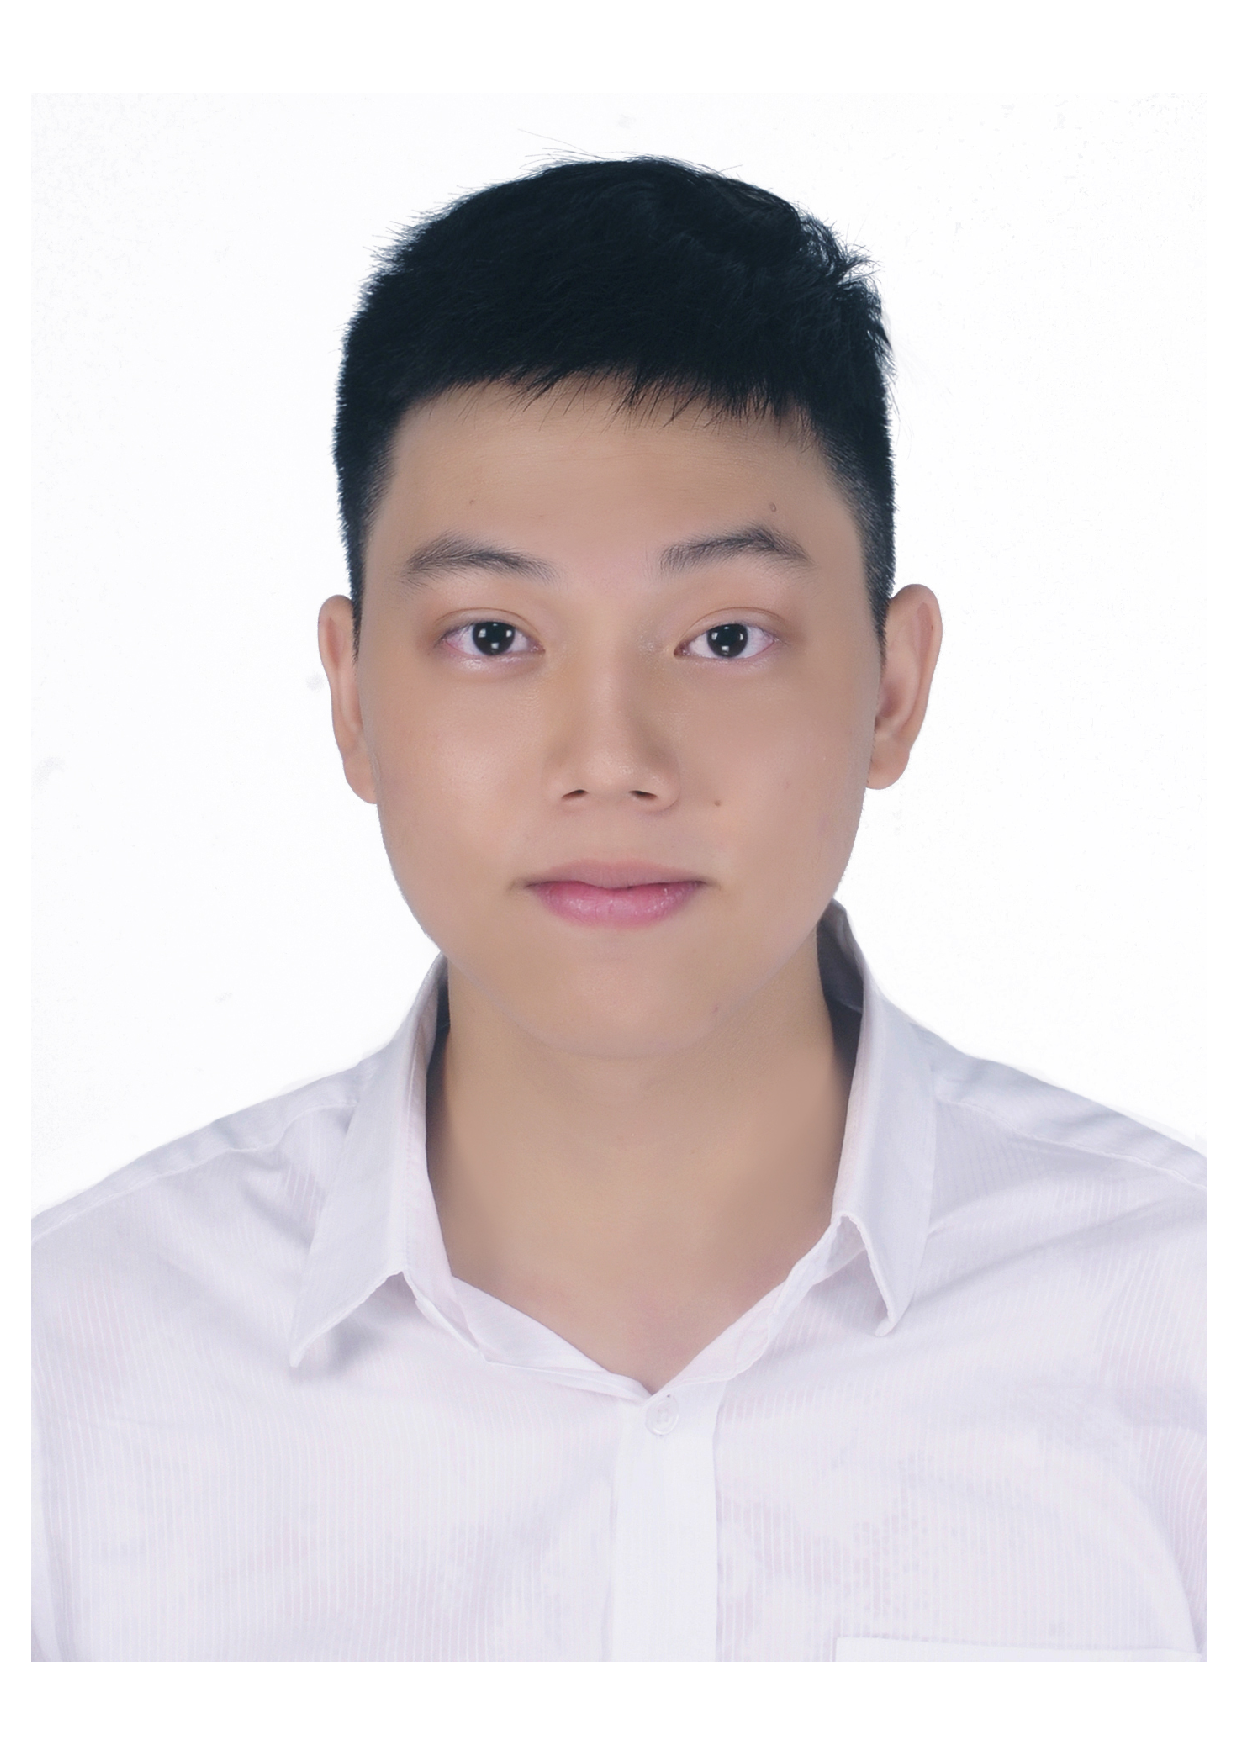
\includegraphics[width=0.6\columnwidth]{photo}
	\vspace{-7cm}
\end{figure}

\begin{flushright}\small
	LI,HONG-RONG \\
	\url{cobras1597535@gmail.com}  \\
	\url{+886-931196217}
\end{flushright}\normalsize
\framebreak


% Right frame
%%%%%%%%%%%%%%%%%%%%
\Huge\bfseries {\color{RoyalBlue} David LI} \\
\Large\bfseries  Engineering Master Student \\

\normalsize\normalfont

% About me
%\begin{AboutMe}

%\end{AboutMe}

% Experience
\section{Experience}

\subsection{Oct 2017 - prensent, National Cheng Kung University}
\subsubsection{Position}
Teaching Assistance
\subsubsection{Content}
Teach the senior about control experiment

\subsection{Oct 2015 - Aug 2016, Taiwan Molex}
\subsubsection{Position}
Engineering Assistance
\subsubsection{Content}
Draw connectors as required
%\SmallSep

\subsection{Aug 2014 - Aug 2015, Starbucks}
\subsubsection{Position}
Barista
\subsubsection{Content}
Making good coffee
%\Sep

\subsection{Apr 2013 - Sep 2013, Thai Town}
\subsubsection{Position}
Waiter
\subsubsection{Content}
Serving food

% Education
\section{Education}

\subsection{2017 - present, National Cheng Kung University}
\subsubsection{Dept.}
Aerospace Engineering
\subsubsection{Degree}
M.S. Degree
\subsubsection{Specialty}
Control

\subsection{2013 - 2017, Tamkang University}
\subsubsection{Dept.}
Aerospace Engineering
\subsubsection{Degree}
B.S. Degree

% Skills
\section{Technical Skills}
\subsection{Coding}
\begin{multicols}{3}
\begin{compactitem}[\color{RoyalBlue}$\circ$] 
	\item C/C++ 
	\item Python
	\item Matlab
\end{compactitem}
\end{multicols}
%\SmallSep
%\item \ldots
\subsection{Markup}
\begin{multicols}{3}
\begin{compactitem}[\color{RoyalBlue}$\circ$]
	\item {\LaTeX} 
	\item Dreamweaver CC 
	\item Office 
\end{compactitem}
\end{multicols}
%\Sep

\subsection{Programming}
\begin{multicols}{3}
\begin{compactitem}[\color{RoyalBlue}$\circ$]
	\item Visual Studio 
	\item OpenCv
	\item LabView 
\end{compactitem}
\end{multicols}

\subsection{Drawing}
\begin{multicols}{3}
\begin{compactitem}[\color{RoyalBlue}$\circ$]
	\item Solidworks 
	\item CATIA
	\item ProE
	\item Autocad
	\item \ldots
	\item \ldots
\end{compactitem}
\end{multicols}

\clearpage
\framebreak
\framebreak

\section{About me}
%\begin{multicols}{2}
\raggedright
\hspace*{5mm}I take this as a precious opportunity to introduce myself to you.\\My name is Hong Rong Li, who majors in aerospace engineering in Tamkamg University. Due to the impoverished family, I have applied\\for Student Loan since I was a senior high school student. Accordingly,\\I am much more ambitious on the aspect of being the top for the\\future success.
\\
\hspace*{5mm}With the globalization, linguistic ability is far more essential in modern society. Therefore, it’s a great advantage for me to possess skillful English ability. Among the my advantages, the best one to make me proud of is my logical thoughts. This can help me choose the most appropriate decision in my lives with deliberate thinking. Besides, I believe that an ordered person can have more leisure time to take advantage of.
\\
\hspace*{5mm}About my particular field, Aerospace Engineering. I will definitely spare no effort to understand thoroughly on my schoolwork. Thus, I had been being on the top three in my department when I was a college student. Speaking of my work experience, Molex is the most significant job to me. What I had learned from it benefited a lot for me, including etiquette, ability of problems solution, self-control and so on.
\\
\hspace*{5mm}I highly eager to be the candidate of exchange student to broaden my horizontal. There are several reasons why you should select me. First of all, I’m more willing as well as diligent to learn about the knowledge from any professional field. Not only did I look up for books from library to get more details, but I attended the class online, Coursera, for more information. Moreover, I stick to my goal, being a specialist at this aspect. That is, I’ll definitely be perseverant whatever adversity I meet in the future. Lastly, I have more pressure resistant than general people due to my living background; therefore, it is not easily for me to surrender to the obstacles.
\\
\hspace*{5mm}By the above-mentioned, I really hope that you have an initial recognition of me, and give me a chance to exchange and discuss\\with faculties at your university. I’ll prove myself to achieve your standard as hard as possible.
%\end{multicols}
\newpage
\framebreak
\framebreak
\section{English Certificates}
\subsection{TOEIC}
\subsubsection{Total score}
895
\Sep
% Usage: 
% \wheelchart {<value1>/<colour1>/<label1>, ...} {Name} {innerRadius} {outerRadius} {innerStrokesColor} {outLinesColor}
\begin{center}
\wheelchart{44.7/antiquewhite/Reading:400,  55.3/antiquewhited/Listening:495}{}{0.5cm}{1.5cm}{gray}{gray}
\end{center}

\subsection{TOEFL iBT}
\subsubsection{Total score}
70
\Sep

\begin{center}
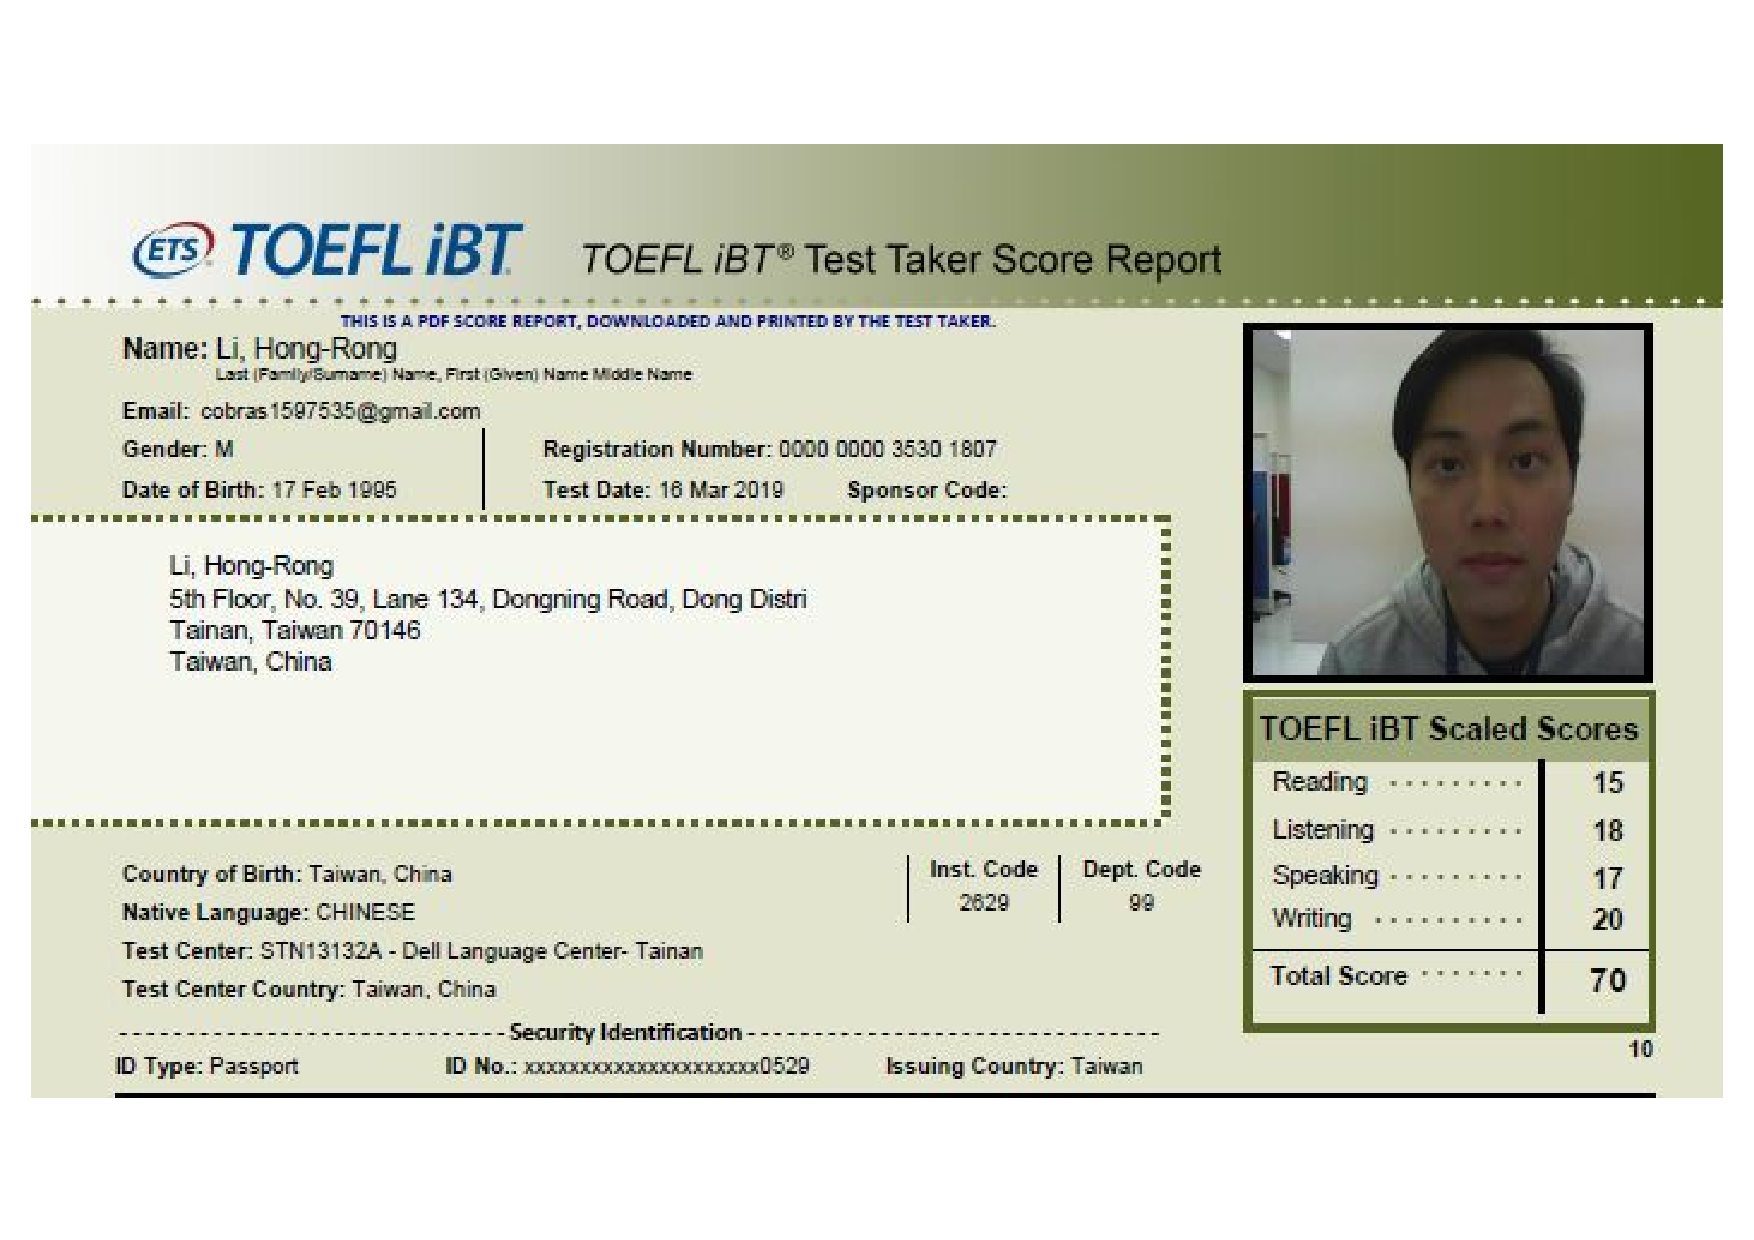
\includegraphics[scale=0.5]{toefl_score.pdf}
\end{center}

\newpage
\framebreak
\framebreak

\section{Application Form}
\begin{center}
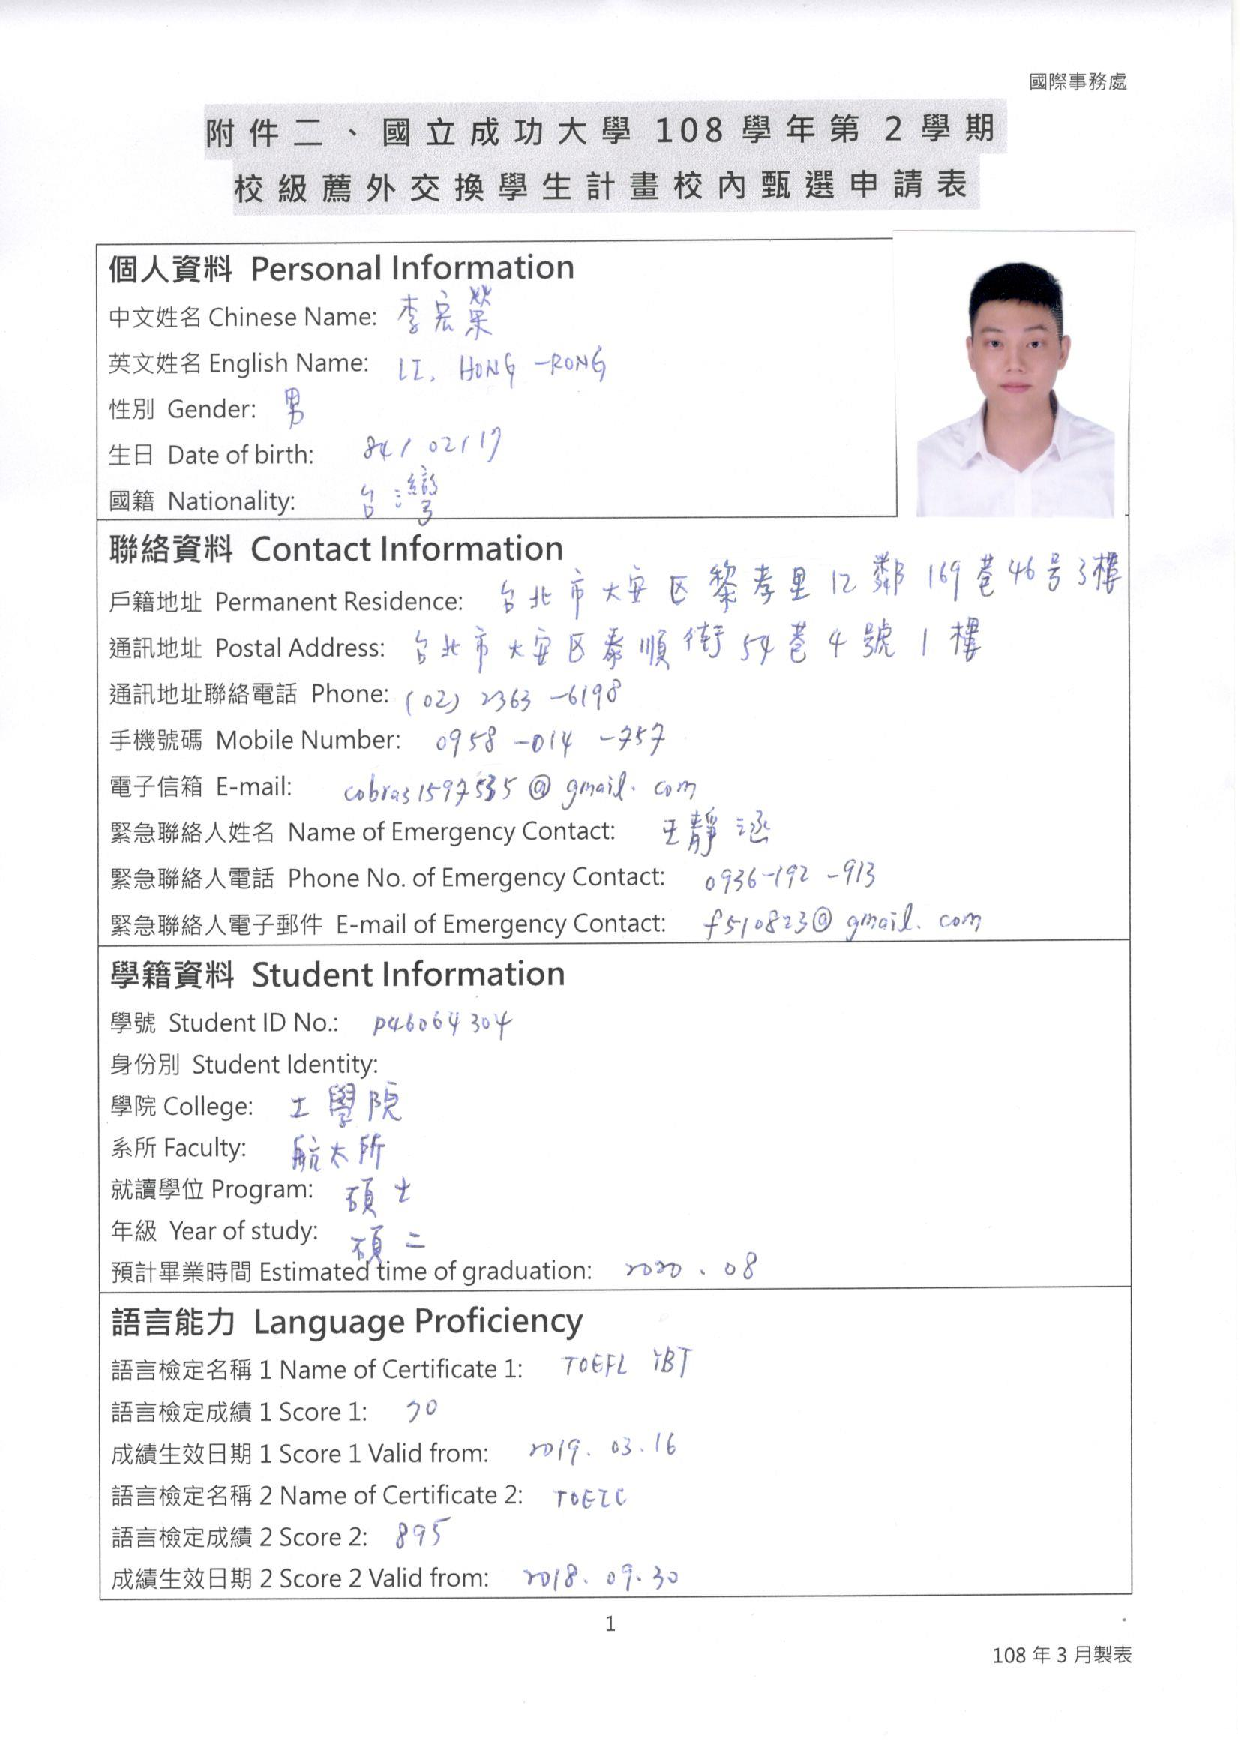
\includegraphics[scale=0.75]{application_form_1.pdf}
\end{center}

\newpage
\framebreak
\framebreak

\section{Application Form - Continue}
\begin{center}
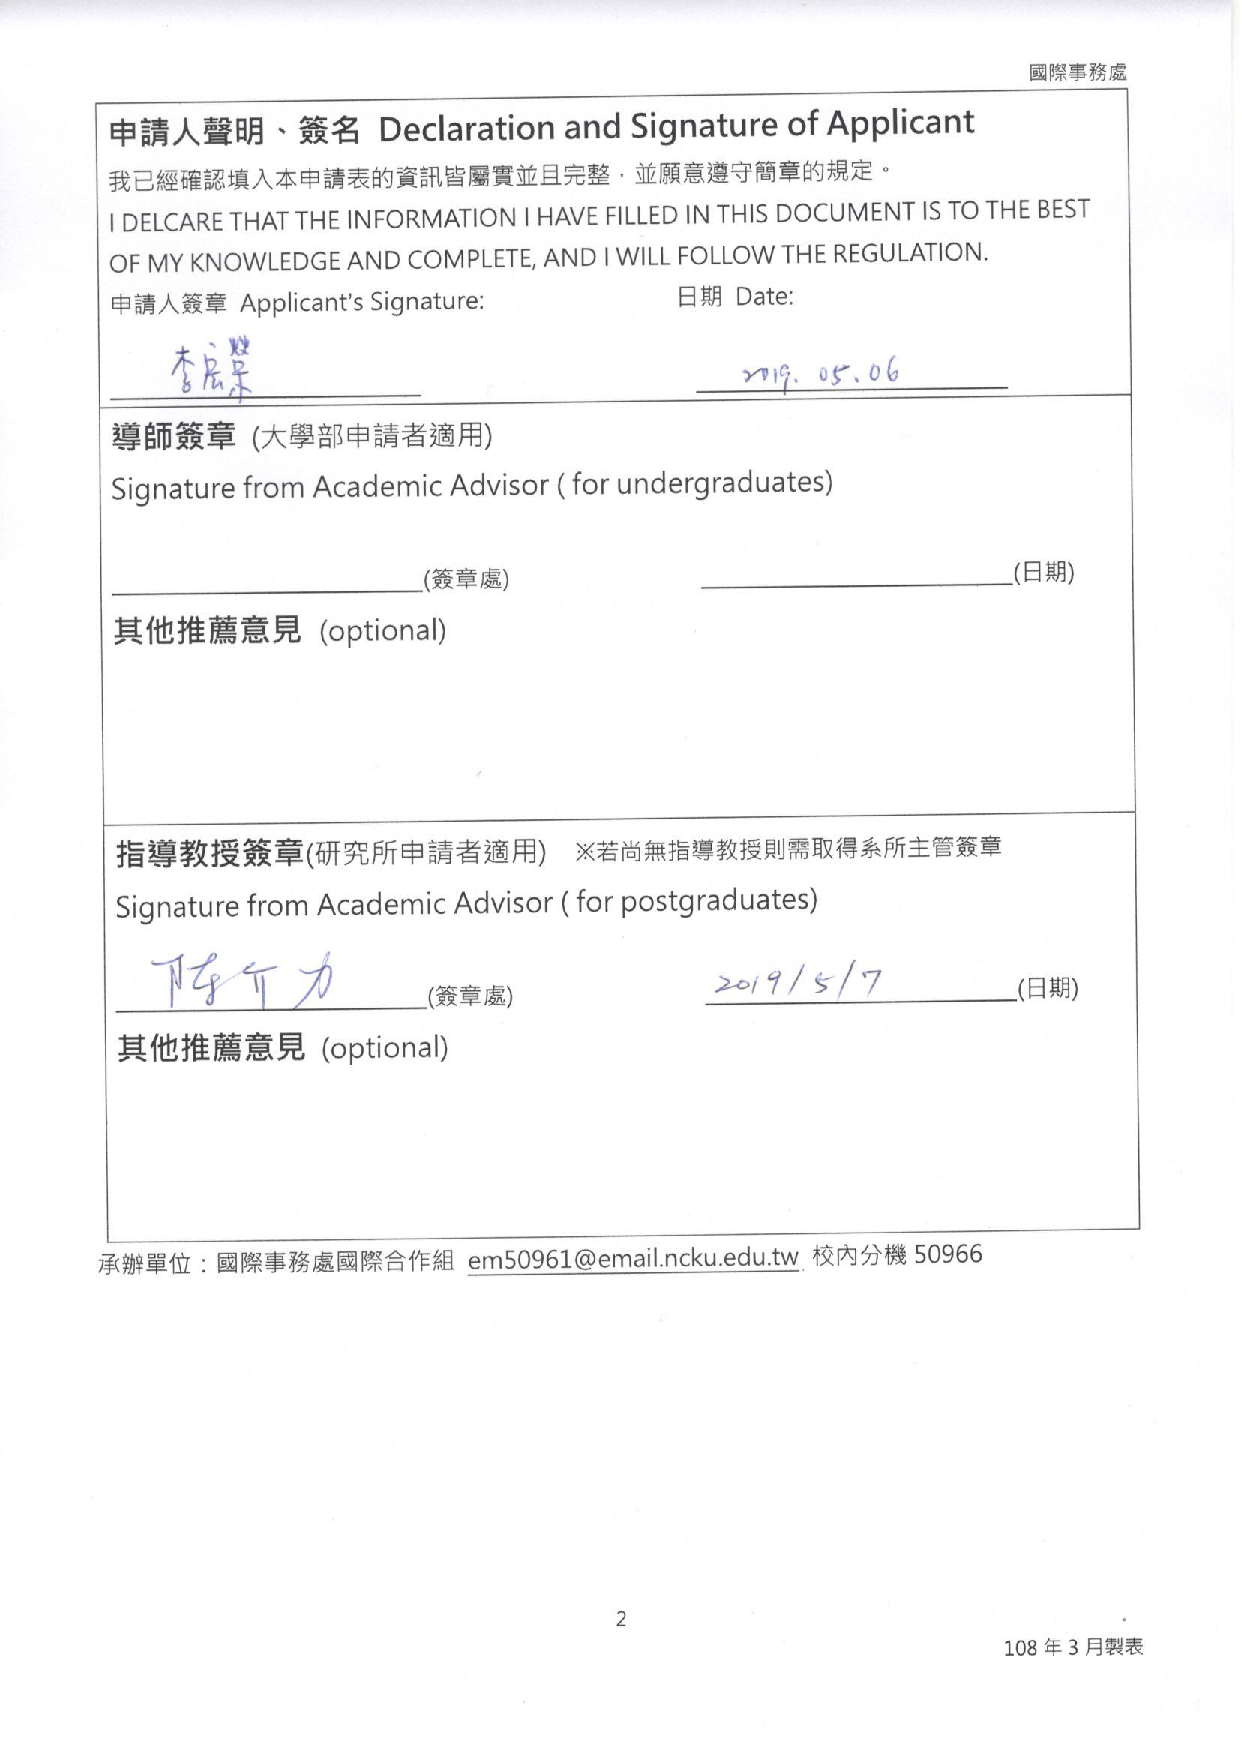
\includegraphics[scale=0.75]{application_form_2.pdf}
\end{center}

\newpage
\framebreak
\framebreak

\section{Grade Transcript}
\begin{center}
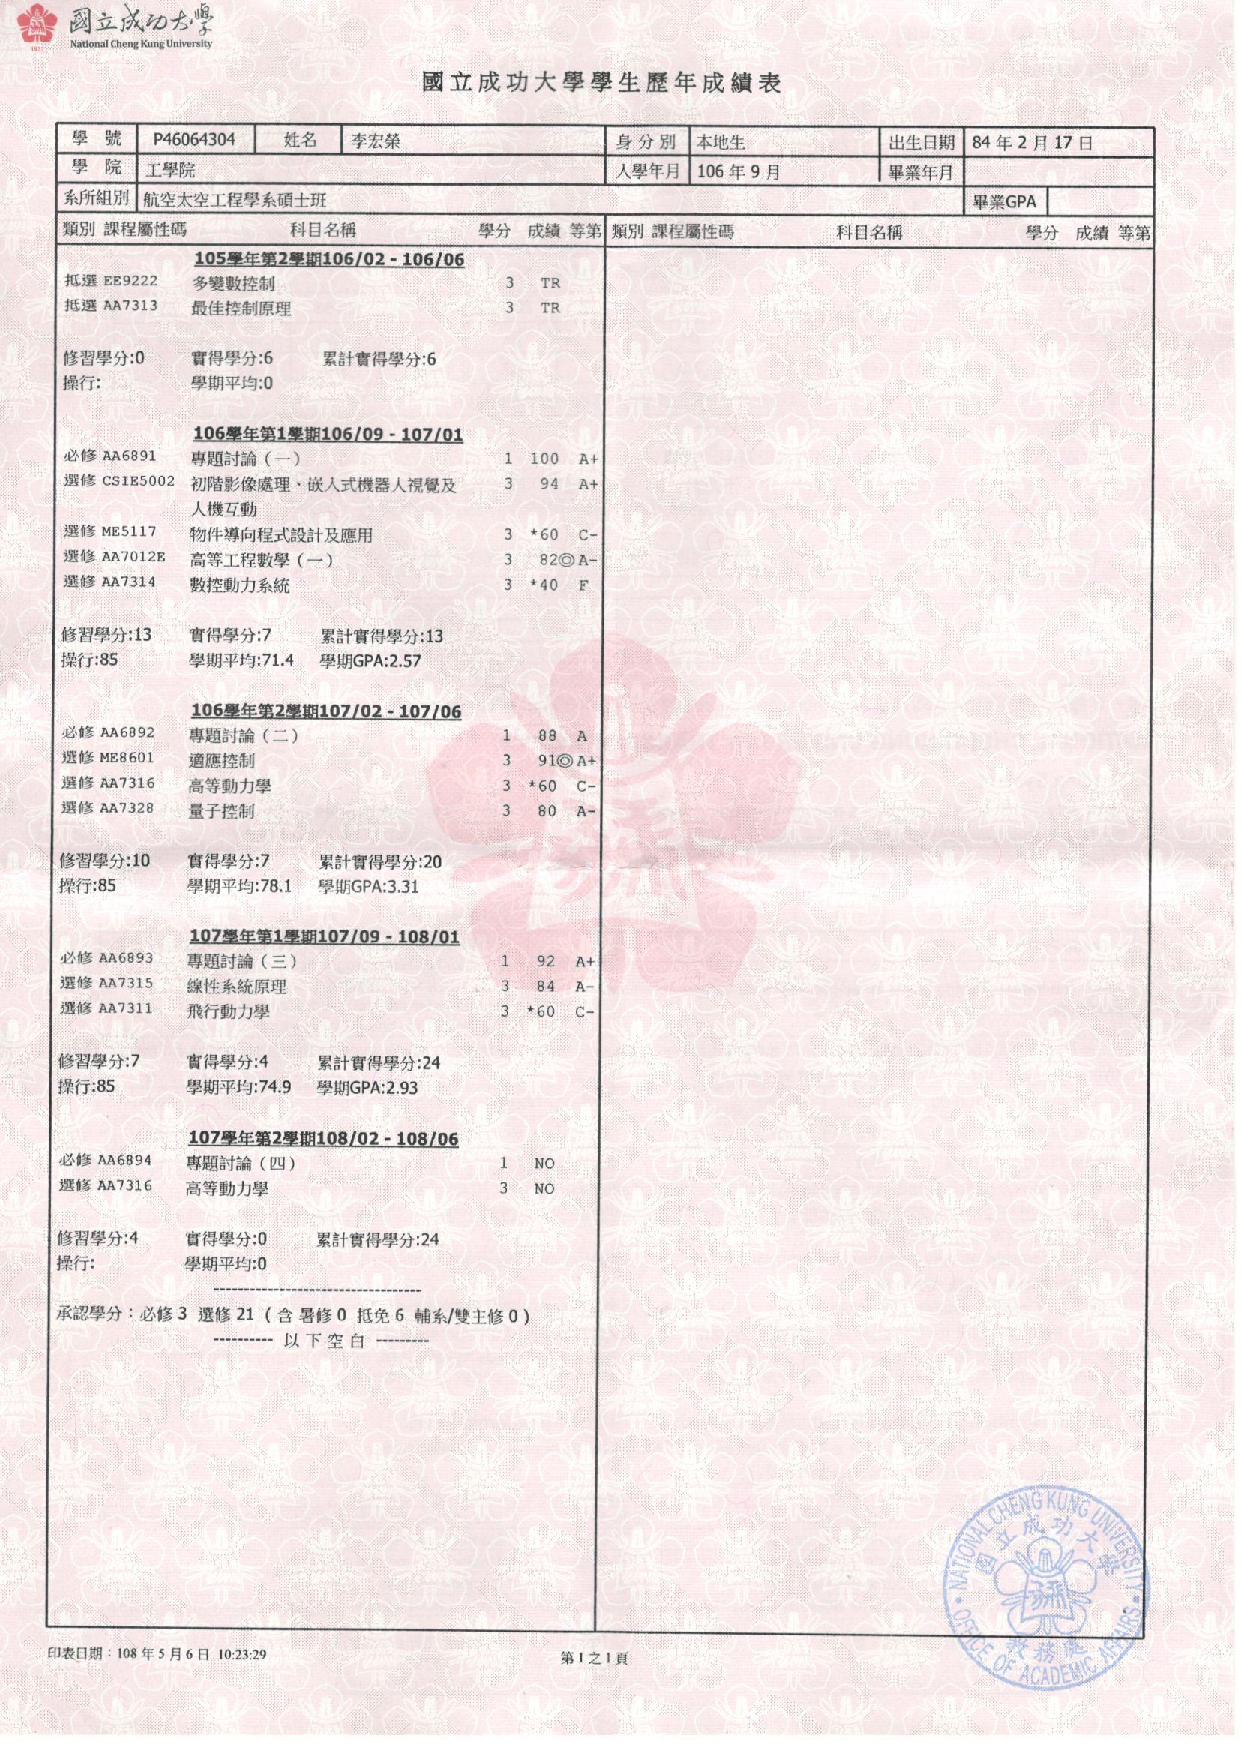
\includegraphics[scale=0.75]{grade.pdf}
\end{center}

\newpage
\framebreak
\framebreak

\section{Research}
\subsection{SLAM For Autonomous Ground Vehicles}
See the attached 1
\attachfile{C:/Users/LAB5892A/Desktop/outgoing/Research_plan/attached_1.pdf}

\section{Publication}
\subsection{Control Of Inverted Pendulum}
See the attached 2
\attachfile{C:/Users/LAB5892A/Desktop/outgoing/Research_plan/attached_2.pdf}

\subsection{Model And Precise Control Of Heat Exchanger}
See the attached 3
\attachfile{C:/Users/LAB5892A/Desktop/outgoing/Research_plan/attached_3.pdf}

\subsection{Final Project Of Advanced Dynamics}
See the attached 4
\attachfile{C:/Users/LAB5892A/Desktop/outgoing/Research_plan/attached_4.pdf}

%%%%%%%%%%%%%%%%%%%%%%%%%%%%%%%%%%%%%
% End document
%%%%%%%%%%%%%%%%%%%%%%%%%%%%%%%%%%%%%
\end{document}